\documentclass{article} % For LaTeX2e
\usepackage{nips15submit_e,times}
\usepackage{hyperref}
\usepackage{url}
\usepackage[pdftex]{graphicx}
%\documentstyle[nips14submit_09,times,art10]{article} % For LaTeX 2.09


\title{Classification of EEG Signals based on Visual Stimuli}


\author{
David S.~Hippocampus
Department of Computer Science\\
Cranberry-Lemon University\\
Pittsburgh, PA 15213 \\
\texttt{hippo@cs.cranberry-lemon.edu} \\
\And
Sandeep D'souza \\
Carnegie Mellon University \\
Address \\
\texttt{email} \\
\And
Coauthor \\
Affiliation \\
Address \\
\texttt{email} \\
\And
Coauthor \\
Affiliation \\
Address \\
\texttt{email} \\
\And
Coauthor \\
Affiliation \\
Address \\
\texttt{email} \\
(if needed)\\
}

% The \author macro works with any number of authors. There are two commands
% used to separate the names and addresses of multiple authors: \And and \AND.
%
% Using \And between authors leaves it to \LaTeX{} to determine where to break
% the lines. Using \AND forces a linebreak at that point. So, if \LaTeX{}
% puts 3 of 4 authors names on the first line, and the last on the second
% line, try using \AND instead of \And before the third author name.

\newcommand{\fix}{\marginpar{FIX}}
\newcommand{\new}{\marginpar{NEW}}

%\nipsfinalcopy % Uncomment for camera-ready version

\begin{document}
\newcommand{\quotes}[1]{``#1''}

\maketitle

%\begin{abstract}
%The abstract paragraph should be indented 1/2~inch (3~picas) on both left and
%right-hand margins. Use 10~point type, with a vertical spacing of 11~points.
%The word \textbf{Abstract} must be centered, bold, and in point size 12. Two
%line spaces precede the abstract. The abstract must be limited to one
%paragraph.
%\end{abstract}

\section{Introduction}

For the course project, we wish to study the correlation of neural signals, to simple tasks performed by humans (for eg., object recognition). The use of machine learning to identify and classify the state of the brain is widely used in the domain of neuroscience. This problem area is particularly useful in the context of brain-computer interfaces, for designing prosthetics, where neural signals (like EEG), need to be classified and translated into the correct action.  Data processing and machine learning have proven very effective in predicting motor motion based on observed EEG signals (Sajda et al., 2003; Lotte et al., 2007) []. The use of machine learning techniques for visual EEG experiments is not as well studied as EEG data in motor movement. For this context, the  EEG response elicited from different object stimuli is likely less regular. The information gleaned from such a study is of interest to neuro-scientists, and can help better understand the visual cognition process [].

\subsection{Datasets and Programming Environment}

In order to learn the dependence of EEG signals on the activity performed by the person, we use the data presented in \cite{eeglab}. This data set contains EEG sensor readings (31 channels sample at 1000 Hz) for an animal categorization task for fourteen different subjects. For each subject, ten sets of animal categorization experiments were conducted. In each experiment the participants were shown hundred images, and asked to categorize the image into 'animal' and 'non-animal' categories. The time stamped EEG sensor data is processed and converted into a workable representation using a Matlab based signal processing toolbox (EEGLAB \cite{eeglab}), that was developed by the same team of researchers who collected the data. The toolbox provides multiple options of data representation (in both the frequency and time domains), which in itself, could be worth investigating as part of the project. The url for the dataset is  $http://sccn.ucsd.edu/~arno/fam2data/publicly\_available\_EEG\_data.html$.

We use both Matlab and python to develop different classifiers for the project. We chose python because of our familiarity with the language and the vast selection of libraries to choose from. Since this project is similar in spirit to the \quotes{Deep Learning meets Neuroscience} project, we would also be using the \textit{TensorFlow} package from Google to implement Convolution Neural Networks (CNNs), among other classification schemes. We use Matlab to leverage the strength of the EEGLAB signal processing tool box, which provides specialized functionality to pre-process EEG signals. 

For the purpose of this project, we need to establish a baseline to compare the accuracy of different classification techniques. For this purpose, we have implemented the Independent Component Analysis (ICA) and Support Vector Machine (SVM) based classification technique presented in [].

\subsection{Baseline}
In [], Stewart et. al. presented an ICA and SVM based approach for single-trial classification of EEG in a visual object task. The work is based on the premise that different visual object stimuli can elicit a response in the brain, which can be detected using EEG recordings. The work in this paper, focuses on classifying whether an EEG signal corresponds to a particular visual stimuli or not. In the experiments presented in the paper, the subjects were asked to label trials as either ‘object present’ or ‘object absent’. This data was then used to train an SVM classifier
and assess the model’s accuracy at labeling subsequent unseen EEG data correctly. Classifier task-labelling accuracy was used as a metric of accuracy. 

\section{SVM based EEG classification}
In this section, we illustrate the details of the technique proposed in [].

\subsection{Data pre-processing}
Data pre-processing is an important step for eeg signal classification tasks. The benefits of pre-processing include removing noise and artifacts that are not relevant to the classification process. In [14], the processing of the raw EEG data was performed using the EEGLAB toolbox \cite{eeglab} in MATLAB. The EEG data was loaded using left mastoid reference, and re-referenced to an average reference later. A Hamming-windowed FIR band-pass filter of 0.1–80 Hz was applied to the EEG data. This is done to remove high frequency noise outside the frequency band of interest. The 1000 Hz recording was downsampled to a sample rate of 250 Hz. This reduces the dimensionality of the data used for classification.
Data rejection was performed by eliminating channels which contained noise above a threshold. Noise of four times that of the median was chosen as a threshold. Electrodes with values exceeding this criterion, are considered noisy and were removed from subsequent analysis.

\subsection{Feature Selection}
To improve the accuracy of classifiers like SVM, it is essential to extract a set of relevant features from the EEG data. In [], two different types of features were used, and the accuracies obtained by using them were compared. The two types used were:

\begin{itemize}
	\item Filtered EEG data
	\item Independent Component Analysis (ICA) activations of the EEG data
\end{itemize}

The first approach involves passing the eeg signal through a band pass filter that only selects waves in the alpha band range - which has been found to be the most important brain signals involved in motor control events.

ICA is typically used for identifying and removing noisy electrodes, blinks and other artefacts to clean up EEG data (Luck, 2005). In [], ICA is used to describe the EEG data, so as to give subsets of data that may be both more interpretable and give higher classifier performance. The ICA components provide an estimation of possible ‘sources’ of generated activity. This can be particularly advantageous in the case of EEG data analysis, where much of the signal (and noise) is shared across all channels (Onton et al., 2006) []. In effect, it can be said that some of the Independent Components (IC) may be useful to describe subsets of variations within the EEG data. 

ICA was applied to the whole dataset from each experimental session, using the Infomax ICA algorithm (Delorme et al., 2007) []. Infomax ICA returns one IC for each electrode

\subsection{Classification}
In classification of EEG, SVMs have been able to present good results (Lotte et al., 2007). Thus, the work in [] uses SVMs as the classifier of choice. The underlying principle of SVM based classification is to solve
a (non-linear) classification problem by transforming it into a linear classification problem in a different, higher dimensional space (or feature space). This is achieved by introducing a non-linear map (feature map)
into the feature space, which can often be an infinite dimensional space of function. In this case the kernel function used  was a radial basis function. The SVM algorithm works by identifying a hyperplane in the transformed feature space that optimally separates the two classes in the training data, giving the maximum margin between the transformed feature points of the two different classes.

For classification, separate classifiers were used for different subjects. In the training phase, a ‘one-versus-one’ SVM model was trained. The classification task was to best label the subsequent data, given this training data. Different SVMs were trained for each the filtered EEG data channels and the Independent Componenets of the data. The voltage time-points from EEG and the independent component (IC) transform activations were normalised before input to the SVM. 

The training data was EEG data/ Independent Components beginning at the time of object presentation until some time after (experimentally varied). For each object, a ‘positive training data’ label was applied to data from trials where an object was shown. Resting baseline EEG data, in which no visual stimuli was displayed (blank screen), was termed ‘negative training data’, where the correct label is ‘object absent’. A flow chart of the technique proposed in [] can be found in Figure \ref{fig:flowchart}.

\begin{figure}
	\centering
	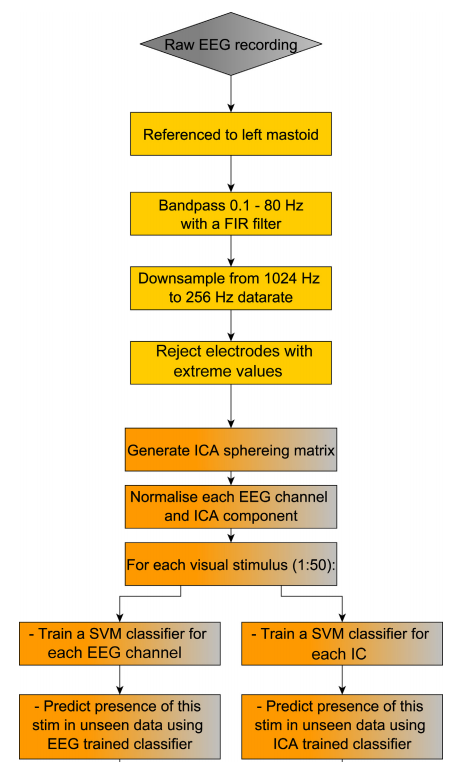
\includegraphics[width=0.5\columnwidth]{flowchart}
	\caption{EEG based Visual Stimulus Classification flow from \textit{A. X. Stewart. et. al. 2014}}
	\label{fig:flowchart}
\end{figure}

\section{Implementation and Experimental Evaluation}
In this section, we illustrate our implementation of the work in [], which we have chosen as our baseline. We implement the scheme in Matlab using some functionality from the EEGLAB toolbox \cite{eeglab}. The different experiments conducted can be broadly classified as follows:

\begin{itemize}
	\item \textbf{Case I:} Using EEG data to classify whether the subject was shown a visual stimulus or not 
	\item \textbf{Case II:} Using EEG data to classify whether the visual stimulus shown to the subject contains an animal or not 
\end{itemize}

Note that, Case I is similar to the objective of the baseline []. For both the problem statements we implement SVM classifiers which use either a single pre-processed EEG channel or a single IC as a feature. We evaluate the implemented techniques on the dataset from \cite{data} (described in Section 1). The evaluations provided are for three subjects, and for each subject we used ten different datasets where the subject had to perform an 'animal categorization' task. For each dataset we use half of the examples to train a classifier and the other half to test the accuracy of the classifier. The accuracy is measured in terms of the percentage of test examples correctly classified. In subsequent sub-sections, we elaborate on the different experiments conducted for the two classification problems.

\subsection{Classifying the Presence of Visual Stimulus}
In this sub-section, we describe the experimental procedure followed in classifying the presence of visual stimuli. Data corresponding to an interval following the instance when the image was shown to the subject is considered as a positive training example, and intervals during which no images were shown is considered to be a negative example (no visual stimulus). For each EEG data channel and IC activation, we train separate SVMs. For both training and classification, based on [] we have chosen two data interval sizes:

\begin{itemize}
	\item Data in the intervals 500 milliseconds, from the instance when the stimulus was applied
	\item Data in the intervals 100 milliseconds, from 75 milliseconds after when the stimulus was applied. These values is based on empirical measurements performed in [].
\end{itemize}
Let the interval size be $T$. For both the EEG channel and IC feature based SVM classifiers, the results for both the interval sizes can be found in Tables 1 \& 2 respectively. For the sake of brevity in the tables we refer to the two classification techniques as EEG-SVM and ICA-SVM. 

\begin{table}[t]
	\caption{Classifying the Presence of Visual Stimulus}
	\label{sample-table}
	\begin{center}
		\begin{tabular}{c|c|cc|cc}
			\multicolumn{1}{c}{\bf Subject } &\multicolumn{1}{c}{\bf Dataset }  &\multicolumn{1}{c}{\bf EEG-SVM} &\multicolumn{1}{c}{\bf EEG-SVM} &\multicolumn{1}{c}{\bf EEG-ICA} &\multicolumn{1}{c}{\bf EEG-ICA}\\
			\multicolumn{1}{c}{\bf }  &\multicolumn{1}{c}{\bf } &\multicolumn{1}{c}{\bf MAX ACCURACY } &\multicolumn{1}{c}{\bf CHANNEL } &\multicolumn{1}{c}{\bf MAX ACCURACY } &\multicolumn{1}{c}{\bf CHANNEL }   
			\\ \hline \\
			cba             &1ff01 &100 & \\
			                &1ff04 &100 &97.49\\
			                &1ff07 &98.94 &86.11\\
			                &1ff10 &100 &95.61\\
			                &1ff13 &100 &89.06\\
			                &2ff01 &100 &86.28\\
			                &2ff04 &97.85 &86.47\\
			                &2ff07 &100 &87.23\\
			                &2ff10 &100 &88.29\\
			                &2ff12 &100 &93.11\\
			\hline  \\
			clm             &1ff01 &64.21 &51.88\\
							&1ff04 &72.34 &52.64\\
			     			&1ff07 &51.58 &51.58\\
			     			&1ff10 &51.54 &50.08\\
			     			&1ff13 &66.31 &51.78\\
			     			&2ff01 &53.84 &53.84\\
			     			&2ff04 &76.34 &53.38\\
			     			&2ff07 &56.04 &53.88\\
			     			&2ff10 &68.08 &52.64\\
			     			&2ff12 &51.57 &51.47\\
			\hline \\
			ega             &1ff01 \\
                 			&1ff04 \\
     						&1ff07 \\
			     			&1ff10 \\
			     			&1ff13 \\
			     			&2ff01 \\
			     			&2ff04 \\
			     			&2ff07 \\
			     			&2ff10 \\
			     			&2ff12 \\
			\hline              
			
		\end{tabular}
	\end{center}
\end{table}

\subsection{Classifying the Type of Visual Stimulus}
In this sub-section, we describe the experimental procedure followed in classifying whether the visual stimuli presented to the subject contains an animal or not. Data corresponding to an interval following the instance when an image containing an animal, was shown to the subject is considered as a positive training example, and intervals during which an image containing no animal was shown, is considered to be a negative example (no visual stimulus). For both of these examples, we consider only instances where the subject was correctly able to identify if the image shown contained or did not contain an animal. For each EEG data channel and IC activation, we train separate SVMs. For both training and classification, based on [] we have chosen two data interval sizes:

\begin{itemize}
	\item Data in the intervals 500 milliseconds, from the instance when the stimulus was applied
	\item Data in the intervals 100 milliseconds, from 75 milliseconds after when the stimulus was applied. These values is based on empirical measurements performed in [].
\end{itemize}







%\section{Work Distribution and Milestones}
%
%In the initial phase of the project, we plan to split the data pre-processing/representation, and the background study phase equally. For the latter part of the project, we would concurrently implement different prospective solutions and compare the results obtained for the implemented classifiers.
%The project milestones we have set are as follows:
%
%\textit{Mid Term} : Data pre-processing, background study and implementation of a simple neural network based classifier. The implemented classifier would classify the activity of the brain based on a small input time-series of the entire data. In this phase we would treat each time-series as independent of the previously data series.
%
%\textit{End Term} : Final implementation of a deep neural network based solution (like RNNs or CNNs), along with the comparisons and results. In this phase, we would try to model the inter-dependence between adjacent time-series. We also wish to incorporate other concepts taught in class such k-fold cross validation, stochastic gradient descent and other optimizations.
%

\section{Future Goals}

For the mid-semester project milestone, we met the goals we set for ourselves. Our mid-semester project goals were:
\begin{itemize}
\item Understanding the state of the art in the field of eeg signal classification
\item Getting familiar with the experiments conducted to collect the data set. We also familiarized ourselves with the data processing tools provided by the research group which collected the data
\item Reproduced the results of a baseline approach selected from published work from 2014
\end{itemize}

Now that we have set up the initial infrastructure required to perform more experiments, we wish to try new methods - introduced in class and mentioned in related work - to improve the classification accuracy. Specifically, we are considering the following directions as the immediate next steps:
\begin{itemize}
\item Try more feature extraction methods, given a fixed classification method, to find the impact of the feature extraction technique on the classification accuracy. Candidates include Power Spectral Density Approaches, Auto regressive coefficients approach and MVAR coefficients approach
\item Try more classification methods that can produce more richer decision surfaces than SVMs. Candidates include - neural networks, decision trees and Logistic regression
\item Explore the effects of concepts introduced in class on the classification accuracy. Candidates include - ensemble methods, cross validation
\item As an ambitious goal to the project, we will apply techniques that improve cross-subject accuracy 
\end{itemize}

%\section{Conclusions}

\bibliographystyle{abbrv}
\bibliography{nips2015}


\end{document}
